\sec{Cloud computing and big data}

\ssec{Why going cloud}

\begin{frame}
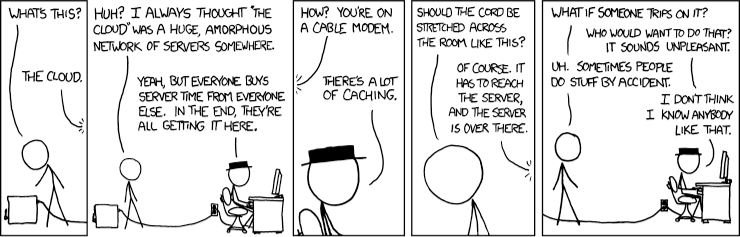
\includegraphics[width=\textwidth]{imgs/xkcd_cloud.png}
\end{frame}


\begin{frame}{Definition}
\begin{block}{Cloud computing (National Institute of Standards and Technology, NIST)}
A model for enabling ubiquitous, convenient, on-demand network access to a shared pool of configurable computing resources (e.g., networks, servers, storage, services) that can be rapidly provisioned and released with minimal management effort or service provider interaction. 
\end{block}

\i On-demand self-service (consume services when you want)
\i Broad network access (consume services from anywhere)
\i Resource pooling (infrastructure, virtual platforms, and applications)
\i Having big pools of resources enables economy of scale
\i Rapid elasticity (enable horizontal scalability)
\i Measured service (pay for the service you consume as you consume)
\end{frame}

\begin{frame}[allowframebreaks]{Why going cloud?}
\textbf{Scalability} that is not possible on premises
\si scale from one server to thousands
of servers
\si grow storage from gigabytes to petabytes
\si no longer think about rack space, switches, and power supplies

\textbf{Reliability} 
\i built to handle failures
\i fault-tolerant or highly available

\framebreak

Service \textbf{integration}
\i services solve common problems (e.g., load balancing, queuing)
\i do not reinvent the wheel

User perspective
\i eliminate repetitive tasks to focus on strategic ones
\i adapt infrastructure to requirements, create (test) environments on demand
\i abstract architecture

Worldwide deployment
\i deploy applications as close to customers as possible
\i improve data locality and privacy
\end{frame}

\begin{frame}{Types of cloud}
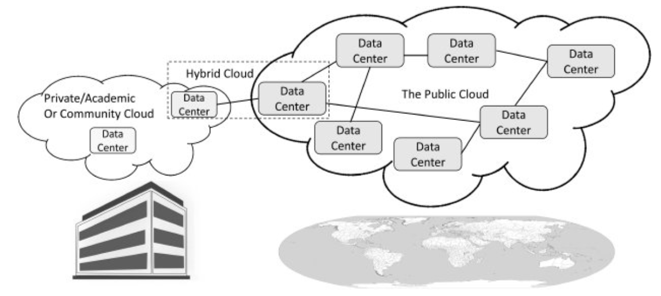
\includegraphics[height=.6\textheight]{imgs/cloud_types.png}
\i Public: accessible to anyone willing to pay (e.g., Microsoft, AWS, Google)
\i Private: accessible by individuals within an institution
\i Hybrid clouds: a mix of the previous
\end{frame}

\begin{frame}{Cloud providers}
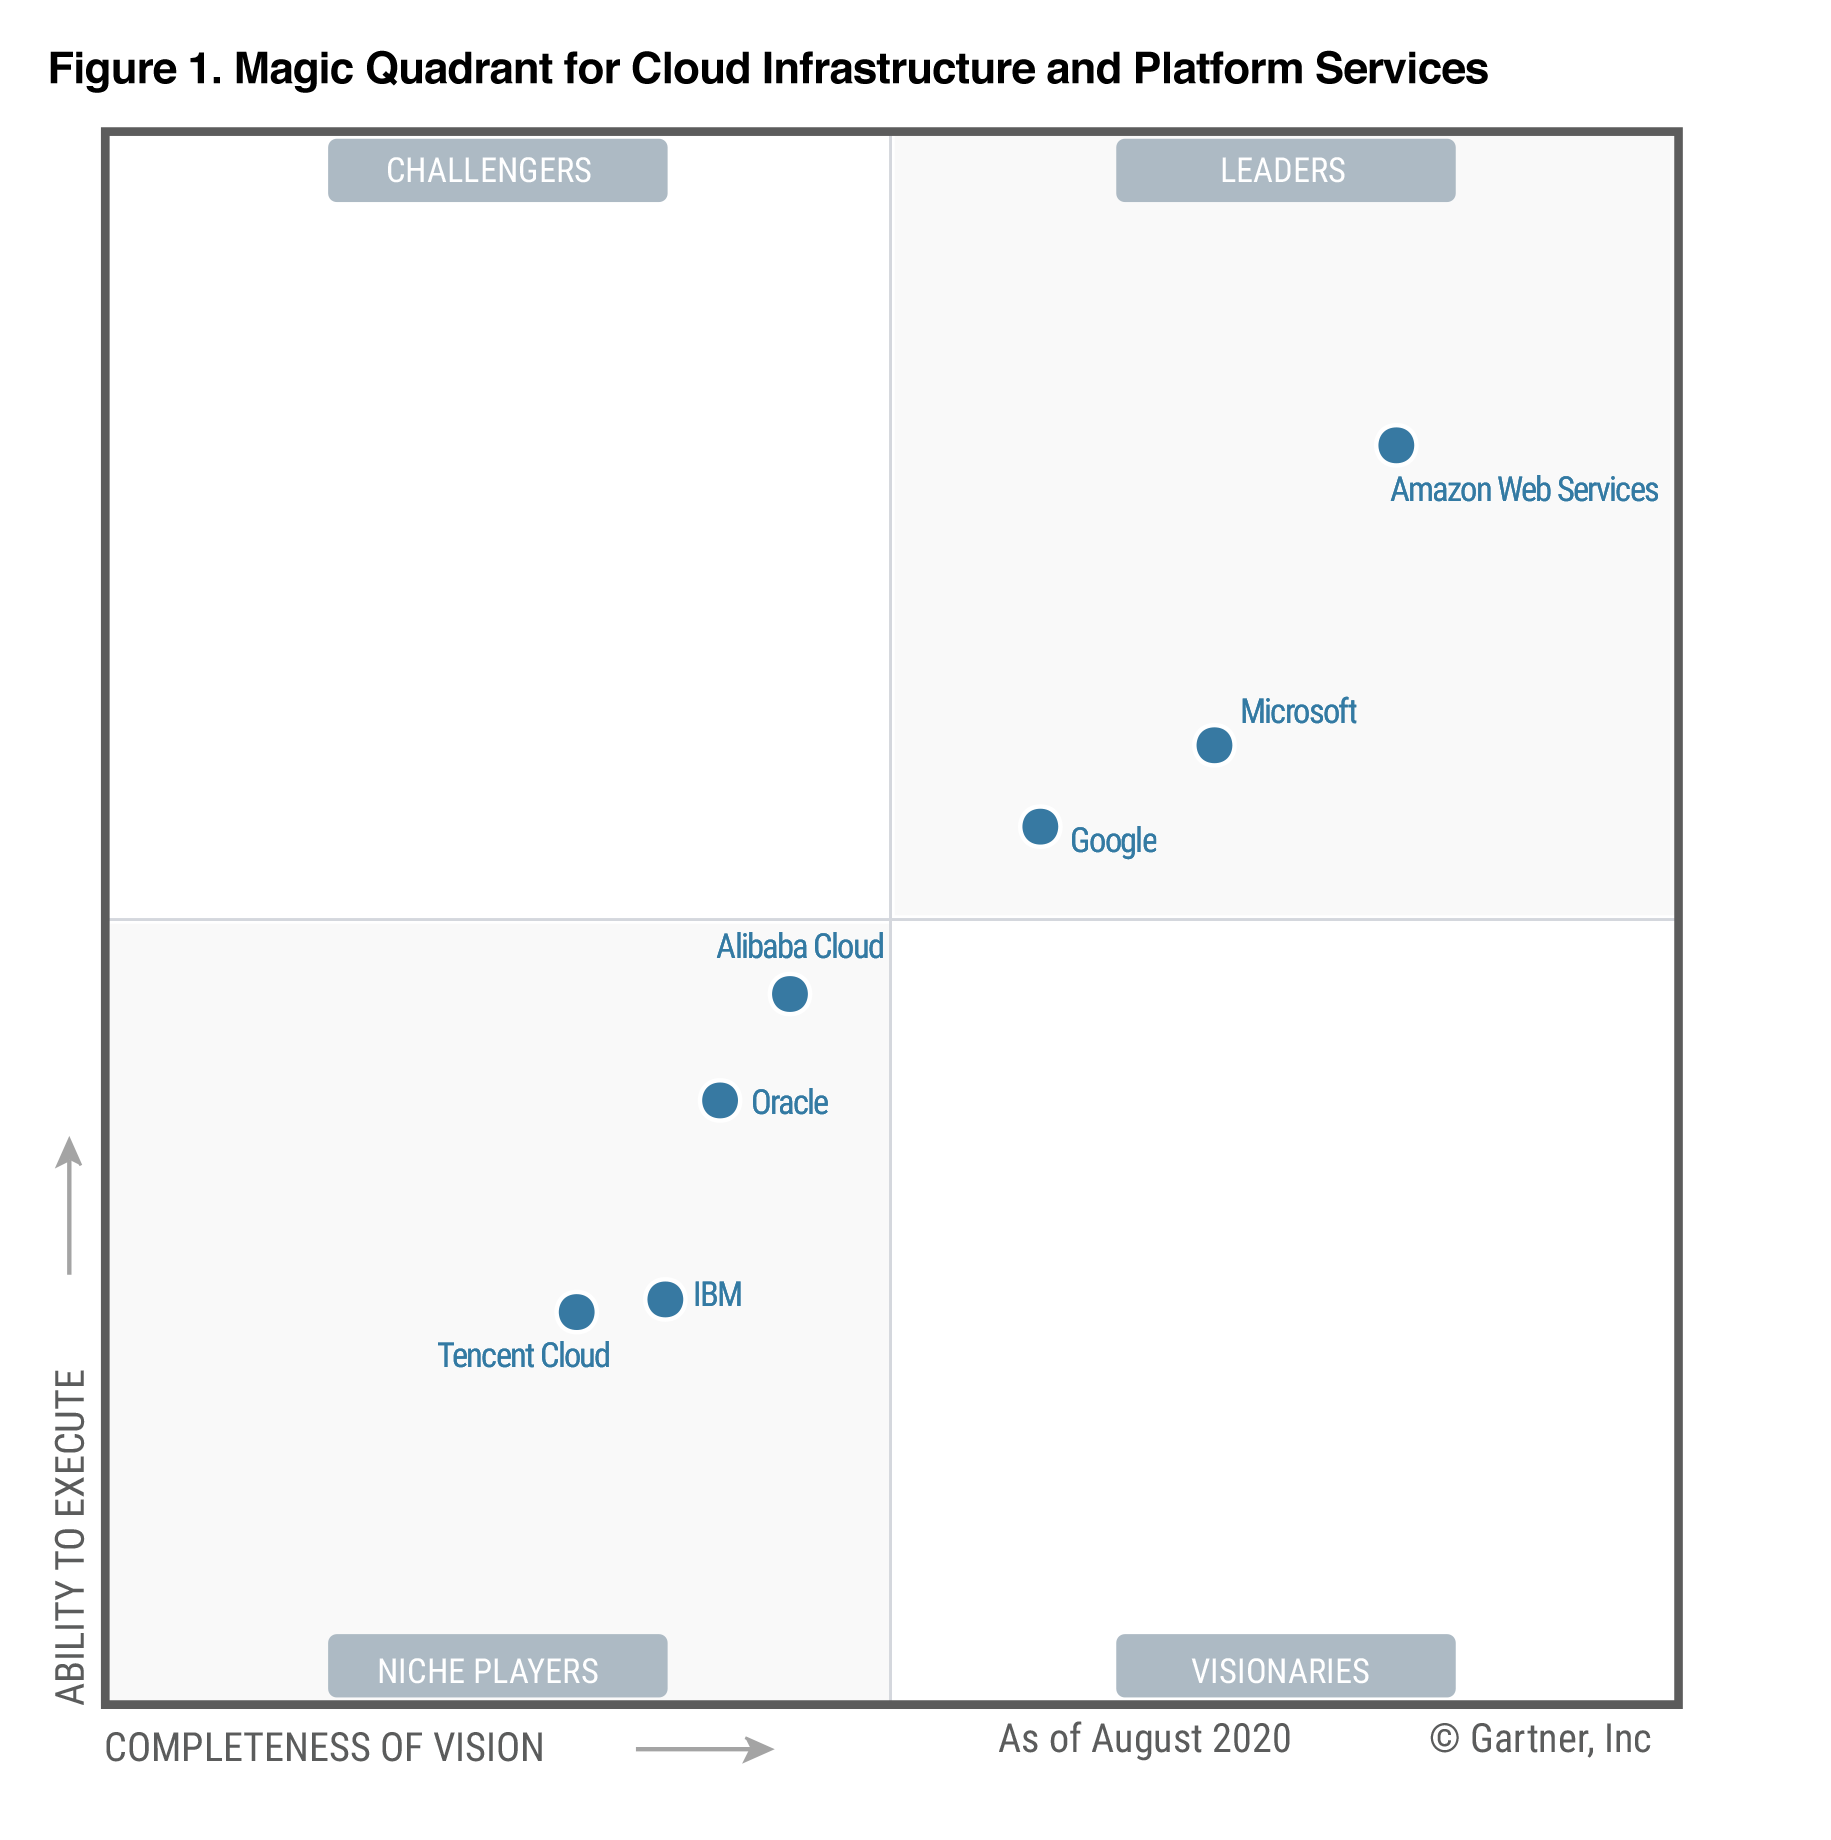
\includegraphics[height=.8\textheight]{imgs/cloud_providers.png}
\end{frame}

\begin{frame}{Types of cloud}
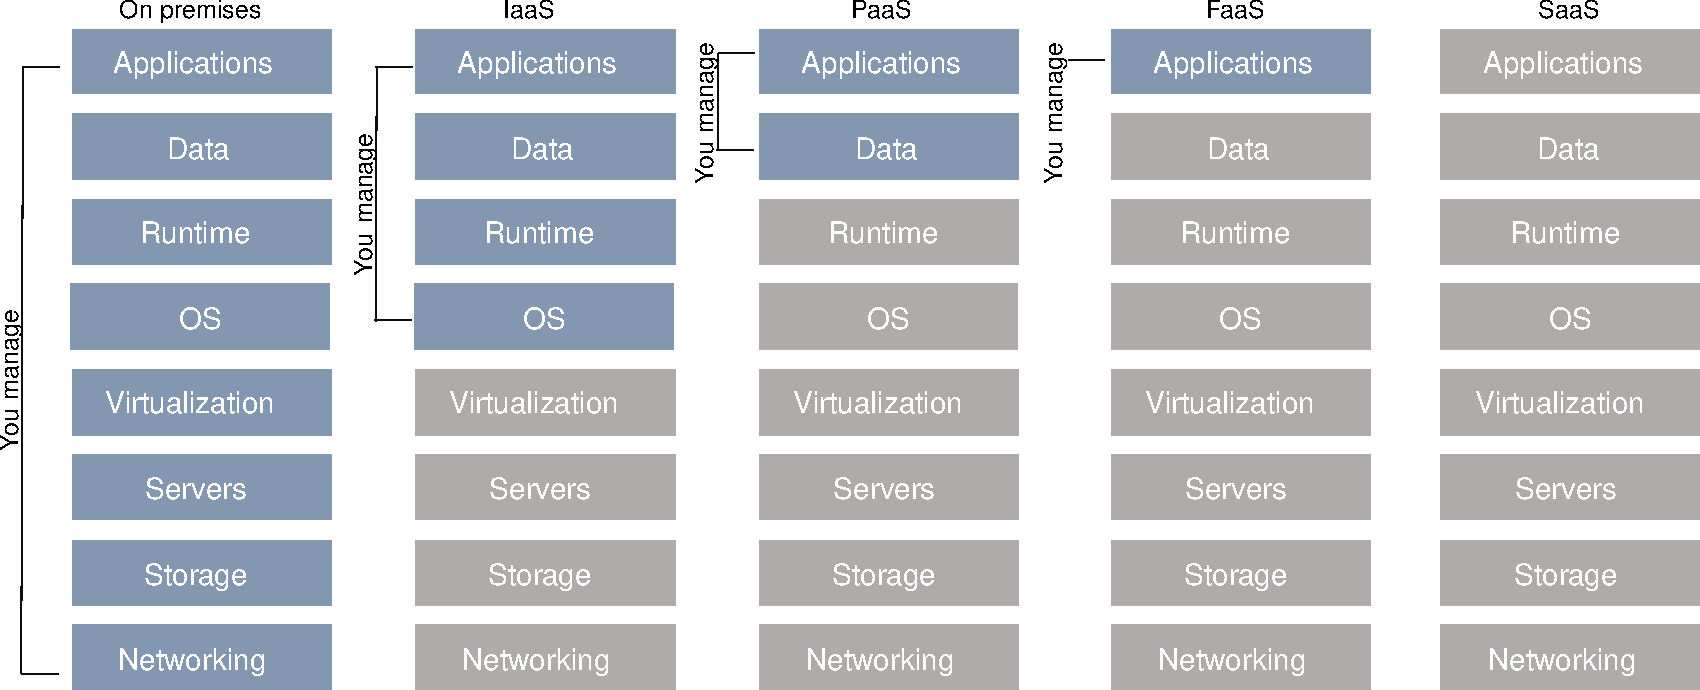
\includegraphics[height=.6\textheight]{imgs/cloud_paastosaas.pdf}
\end{frame}

\begin{frame}[allowframebreaks]{Types of cloud}

Understanding architectures is paramount to successful software systems
\i good architectures help to scale
\i poor architectures cause issues that necessitate a costly rewrite

\textbf{On premises}
\i provisioning, managing, and patching servers is time-consuming
\i require dedicated operations people
\i a non-trivial environment is hard to set up and operate effectively
\i infrastructure and hardware are often a distraction from strategic tasks

\framebreak

\textbf{Infrastructure as a service (IaaS)} 
\i a computing infrastructure provisioned and managed over the internet
\i avoid expense/complexity of buying/managing \textit{physical} servers/datacenters
\i IaaS overcomes issues on premises
\si possibly requires to manage many environments

\textbf{Platform as a Service (Paas)}
\i a development and deployment environment in the cloud
% \i like IaaS, includes infrastructure-servers, storage, and networking
\i support complete application lifecycle: building, testing, deploying, etc.
\i avoid expense/complexity of managing licenses and application infrastructure

\framebreak

\textbf{Function as a Service (FaaS)}
\i a coding environment, cloud provider provisions platform to run the code
\i infrastructure provisioning and management are invisible to the developer
\i avoid to manage infrastructure

\textbf{Software as a service (SaaS)} 
\i an application environment 
\i access cloud-based apps over the Internet (e.g., email, Microsoft Office 365)
\end{frame}

\begin{frame}[allowframebreaks]{From PaaS to FaaS (serverless)}

\textbf{PaaS} and \textbf{containers} are potential solutions to inconsistent infrastructures

\i \textbf{PaaS} provides a platform for users to run their software
\si developers write software targeting features/capabilities of the platform

\i \textbf{containerization} isolates an application with its own environment
\si lightweight alternative to full virtualization
\si containers are isolated but need to be deployed to (public/private) server
\si excellent solution when dependencies are in play
\si "housekeeping" challenges and complexities

% \begin{block}{Microservices}
% Small, standalone, fully independent services built for a specific purpose
% \end{block}
% \i Each service written in an appropriate framework and language
% \si Benefits from the right language/libraries
% \si Many languages and frameworks are hard to support
% \i Each microservice can maintain state and store data
% \si eventual consistency, transaction management, and complex error recovery can make things hard

\framebreak


\textbf{Serverless}
\i a software architecture that does not rely on direct access to a server

FaaS is based on a serverless approach
\i every function could be considered as a standalone service
\i embodies principles from microservices
\si small, standalone, fully independent services built for a specific purpose
\si each service written in an appropriate framework and language
\i cloud provider is responsible for integration 
% \i Many languages and frameworks are hard to support
% \i Each microservice can maintain state and store data

\framebreak

Principles of FaaS/serverless architectures
\i use a compute service to execute code on demand (no servers/containers)
\i write single-purpose stateless functions
\i design push-based, event-driven pipelines
\i create thicker, more powerful front ends
\i embrace third-party services

FaaS/Serverless is not a silver bullet
\i not appropriate for latency-sensitive applications 
\i strict specific service-level agreements
\i vendor lock-in can be an issue for enterprise and government clients
\i should not base mission-critical applications on a public cloud

\framebreak

Write single-purpose stateless functions
\i keep the single responsibility principle in mind
\si a function that does just one thing is more testable and robust
\si a function with a well-defined interface is also more likely to be reused
\i code should be created in a stateless style
\si local resources or processes will not survive along sessions
\si statelessness allows scalability
\i functions that terminate sooner are cheaper 
\si (pricing is based on \#requests, execution time, and allocated memory)
% Having less to do in Lambda is cheaper.  Moreover, building a rich front end (in lieu of a complex back end) that can talk to third-party services directly can be conducive to a better user experience. Fewer hops between online resources and reduced latency will result in a better perception of performance and usability of the application. In other words, you don’t have to route everything through a compute service. Your front end may be able to communicate directly with a search provider, a database, or another useful API.

Compose functions in a loose orchestration
\i build complex but understandable back-end systems
\i event-driven and push-based pipelines
\end{frame}



% \begin{frame}{History in (very) brief}
% Computing as a service is far from new

% \begin{itemize}
% \item 1961, John McCarthy at MIT: "Computing may someday be organized as a public utility just as the telephone system [...] Each subscriber needs to pay only for the capacity he uses, but he has access to all programming languages characteristic of a very large system" 
% \item 1969, UCLA turns on first node of ARPANET. "As [computer networks] grow up and become more sophisticated, computer utilities will spread"
% \item 1990s USA, gigabit testbeds linked research laboratories. "Meta-computer", virtual computational systems created by linking components at different sites
% \item Large Hadron Collider (LHC) federates computing systems at hundreds of sites to analyze PBs of data. LHC Computing Grid enables on-demand access to computing and storage 
% % 2006 Emergence of cloud computing, a story of marketing, business model, and technological innovation
% % \i Cloud is driven by a transformation in demand (First successful IaaS emerged from an e-commerce provider)
% % \i Amazon was building hundreds of similar work-unit computing systems to support different services
% \end{itemize}
% \end{frame}
% \begin{frame}{Data transformation}
% 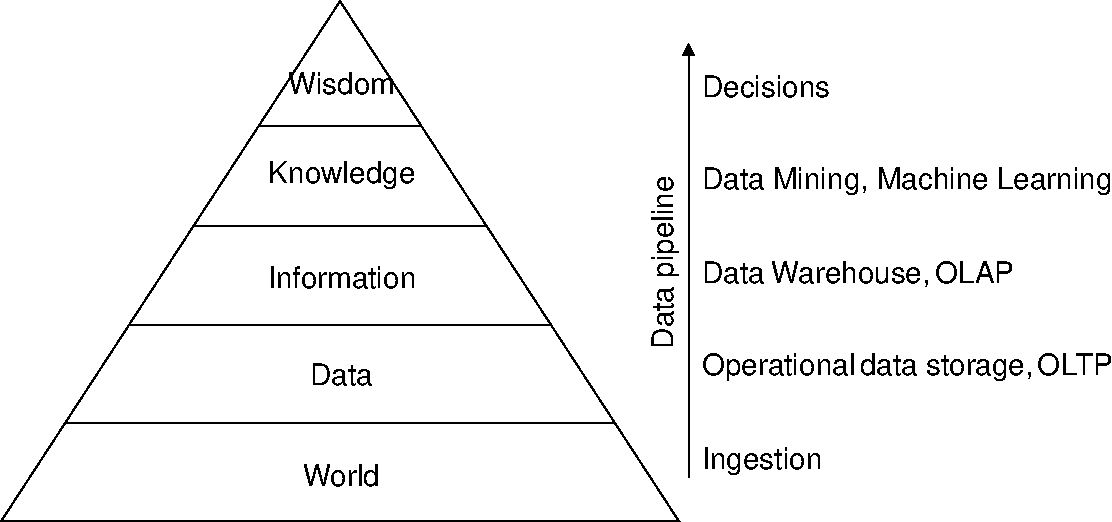
\includegraphics[height=.8\textheight]{imgs/knowledgepyramid.pdf}
% \end{frame}


\ssec{Data pipelines on cloud}

\begin{frame}{}
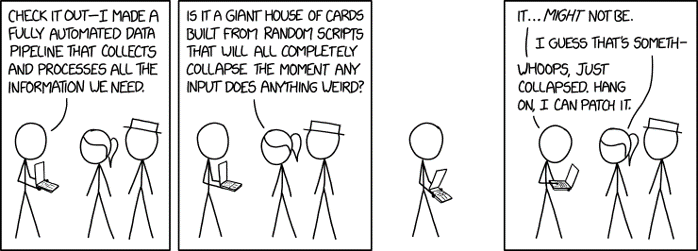
\includegraphics[width=\linewidth]{imgs/xkcd_pipeline.png}    
\end{frame}

\begin{frame}{Date pipelines on cloud}
Architecting data pipelines on cloud requires to \textbf{standardize/integrate} services
\i Make them available through simple portals
\i Track usage/cost with billing mechanism
\i Measure availability
\i Orchestrate to meet demand
\i Provide a security framework
\end{frame}

\begin{frame}{Which services do we need?}
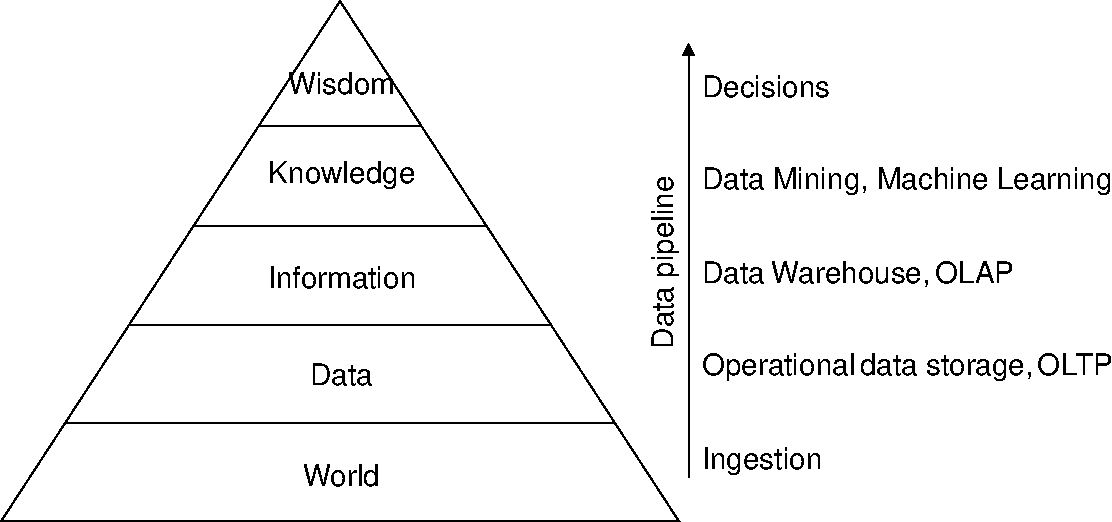
\includegraphics[height=.7\textheight]{imgs/knowledgepyramid.pdf}
\end{frame}

\begin{frame}{How do we organize them?}
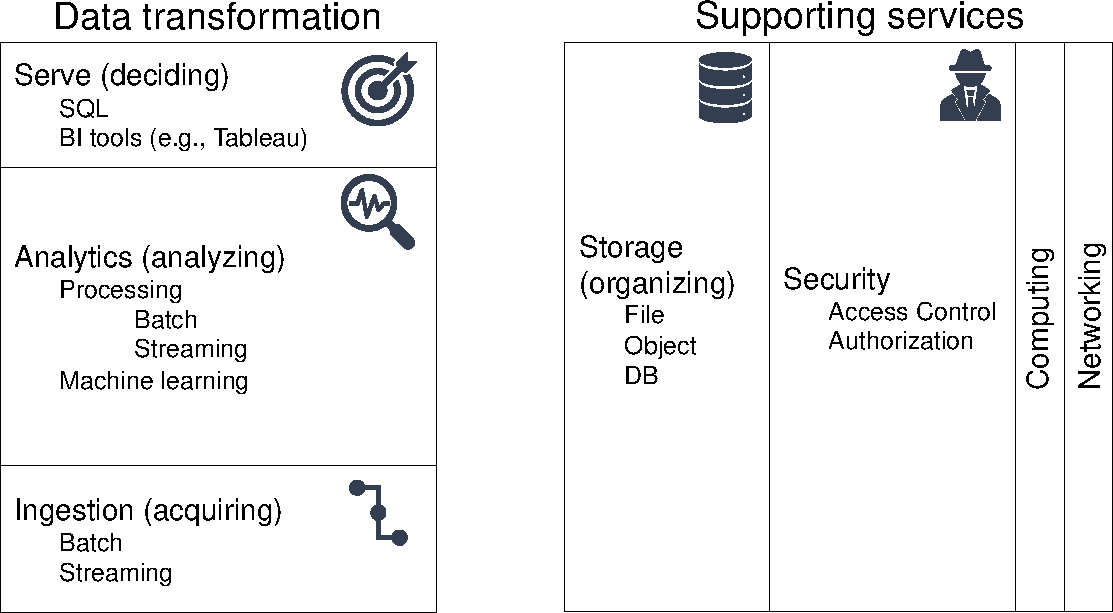
\includegraphics[height=.7\textheight]{imgs/cloudpatchwork.pdf}
% \begin{frame}[allowframebreaks]{At what costs?}
% Physical costs (and economy of scale)
% \si charges for AWS have been reduced 42 times since 2008 (up to 2014)
% \si 12/2014, charges for outbound data transfer were lowered by up to 43\%
% \si 11/2014, charges for search service were lowered by 50\%
% \si 03/2014, charges for virtual server were lowered by up to 40\%


% However, datasets are
% \i From various sources and unstructured (variety) 
% \i Of large size (volume)
% \i With fast data in/out (velocity)

% \textbf{Challenges}: data assimilation, aggregation, classification, etc.
\end{frame}


\begin{frame}{Data pipeline on cloud: AWS}
\url{https://aws.amazon.com/it/architecture/analytics-big-data}
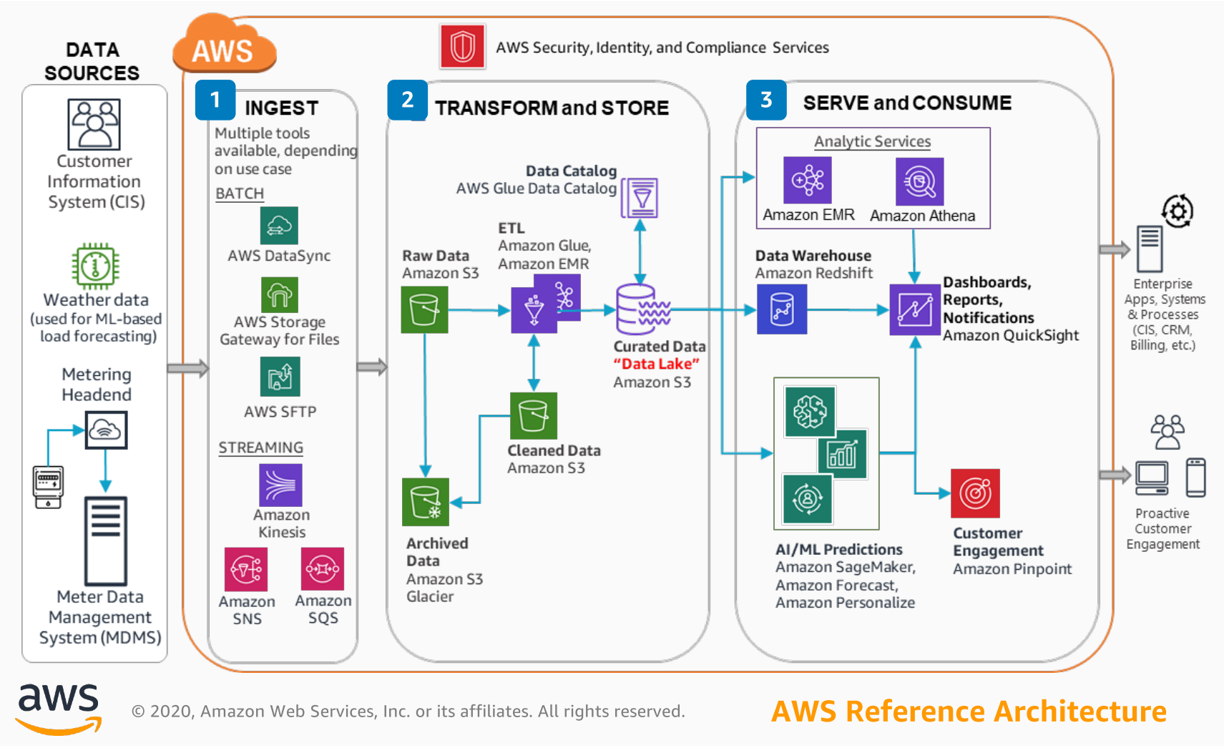
\includegraphics[height=.8\textheight]{imgs/awspipeline.png}
\end{frame}

\begin{frame}[allowframebreaks]{AWS: storage}

\end{frame}


\begin{frame}[allowframebreaks]{Storage}

\textbf{Storage models}
\i Different ways in which data are organized in a storage system

Understand properties of these different storage models to choose the right system
\i The right model depend on nature and size of the data
\i Analyses to be performed
\i Access / Update frequencies
\end{frame}

\begin{frame}[allowframebreaks]{Storage: types of storage models}
\textbf{Types} of storage models
\i File systems (or file storage)
\i Object storage
\i Block storage
\i Relational / NoSQL / Graph databases

\textbf{File system} 
\i stores unstructured binary objects
\i organized around a tree of directories or folders
\i extremely intuitive and useful data storage abstraction
\i disadvantages as a basis for science and engineering, particularly as data volumes grow
\si no support for enforcing conventions concerning the representation of data elements and their relationships
\si rigid hierarchical organization enforced by a file system often does not match the relationships that one wants to capture in science.
\si cannot help users navigate complex data collections
\si need to maintain consistency as multiple processes read and write a file system can lead to bottlenecks

\textbf{Object Stores}
\i like file system model, stores unstructured binary objects
\i objects are often referred to as blobs, for binary large object
\i simplifies the file system model
\si eliminates hierarchy 
\si forbids updates to objects once created
\i in general they support a two-level folder-file hierarchy
\i little support for organizing data and no support for search
\si user must know an object0s identifier in order to access it

\textbf{Databases} 
\i Relational Databases
\i NoSQL Databases
\si key-value
\si columnar
\si document based
\si graph

\begin{table}
    \centering
    \begin{tabular}{llll}
        Model& Amazon& Google& Azure\\
        Files & Elastic File System (EFS), Elastic Block Store (EBS) & Google Cloud attached file system & Azure File Storage\\
        Objects & Simple Storage Service (S3) & Cloud Storage & Blob Storage Service \\
        Relationa& Relational Data Service (RDS), Aurora & Cloud SQL, Spanner & Azure SQL\\
        NoSQL& DynamoDB, HBase& Cloud Datastore, Bigtable & Azure Tables, HBase\\
        Graph& Titan& Cayley& Graph Engine\\
        Warehouse& Redshift & BigQuery& Data Lake\\
    \end{tabular}
\end{table}
\end{frame}

\begin{frame}[allowframebreaks]{Storage: access frequency}
Access frequency determines availability and pricing
\i Standard: optimized for performance and high frequency access
\i Nearline: for data accessed less than once a month
\i Coldline: for data accessed less than once a quarter
\i Archive: most cost-effective, data accessed less than once a year

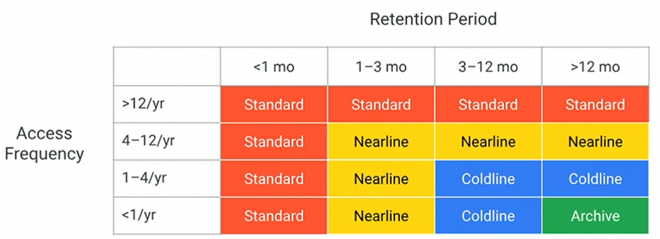
\includegraphics[width=\linewidth]{imgs/gc_accessfrequency.png}
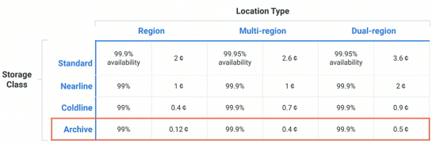
\includegraphics[width=\linewidth]{imgs/gc_accessfrequency_region.png}
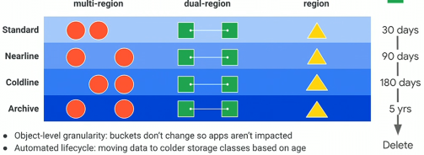
\includegraphics[width=\linewidth]{imgs/gc_accessfrequency_region2.png}
\end{frame}

\begin{frame}[allowframebreaks]{Storage: types of analyses}
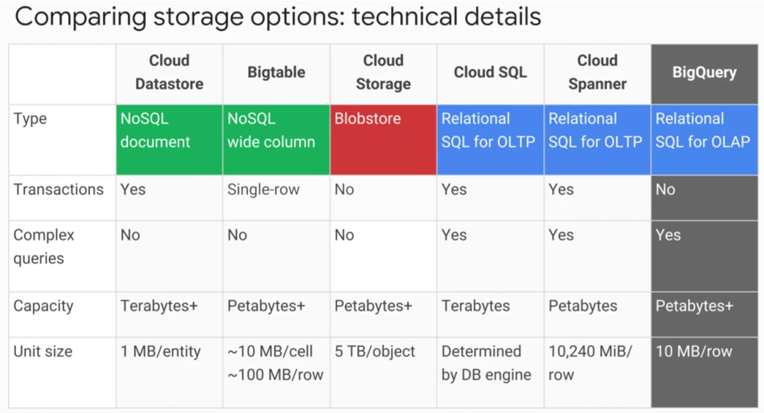
\includegraphics[width=\linewidth]{imgs/gc_storage_analyses.png}
\end{frame}

\begin{frame}[allowframebreaks]{AWS: ingestion}
\textbf{Batch}

\i \textbf{AWS DataSync}
\si move data between on-premises storage and S3/EFS/etc.
\si on-premises software transfers data via Network File System protocol
\si pay only for the data you copy

\i \textbf{AWS Transfer for SFTP} 
\si transfer files in/out Amazon S3 using Secure File Transfer Protocol

Moving data to the cloud
\i \r{80TB} of data to move, \g{1Gbps} connection to the internet
\i \b{How many days}? 
\si \r{80000GB} / \g{(1Gbps / 8)} / \b{60 / 60 / 24} \~= a week without internet


\framebreak

\textbf{Stream}

\i \textbf{Kinesis} 
\si collect, process, and analyze real-time, streaming data
\si ingest real-time data such as video, audio, application logs, etc. 
\si analyze data as it arrives (and not until all data is collected)

\i \textbf{Kinesis Data Firehose}
\si load streaming data into storage/analytics
tools (S3, Elasticsearch, etc.)
\si automatically scales to match the throughput

\i \textbf{Kinesis Data Analytics}
\si analyze streaming data in real time
\si use SQL to continuously query streaming data
\si scales automatically to match the volume and throughput rate

\framebreak

\i \textbf{Simple Queue Service (Amazon SQS)} 
\si message queue that decouples microservices/serverless
\si send/store/receive messages, avoid message loss
\si \textit{Standard}: max. throughput, best-effort ordering, at-least-once delivery
\si \textit{FIFO}: exact ordering, exactly-once delivery

\i \textbf{Simple Notification Service (SNS)}
\si topics for high-throughput, push-based, many-to-many messaging
\si fan out messages to a large number of subscriber endpoints
\end{frame}

{
\bgimg{1}{imgs/awssnowmobile.png}
\begin{frame}{AWS: ingestion}
    
\end{frame}
}

\begin{frame}{Data pipeline on cloud: Google Cloud}
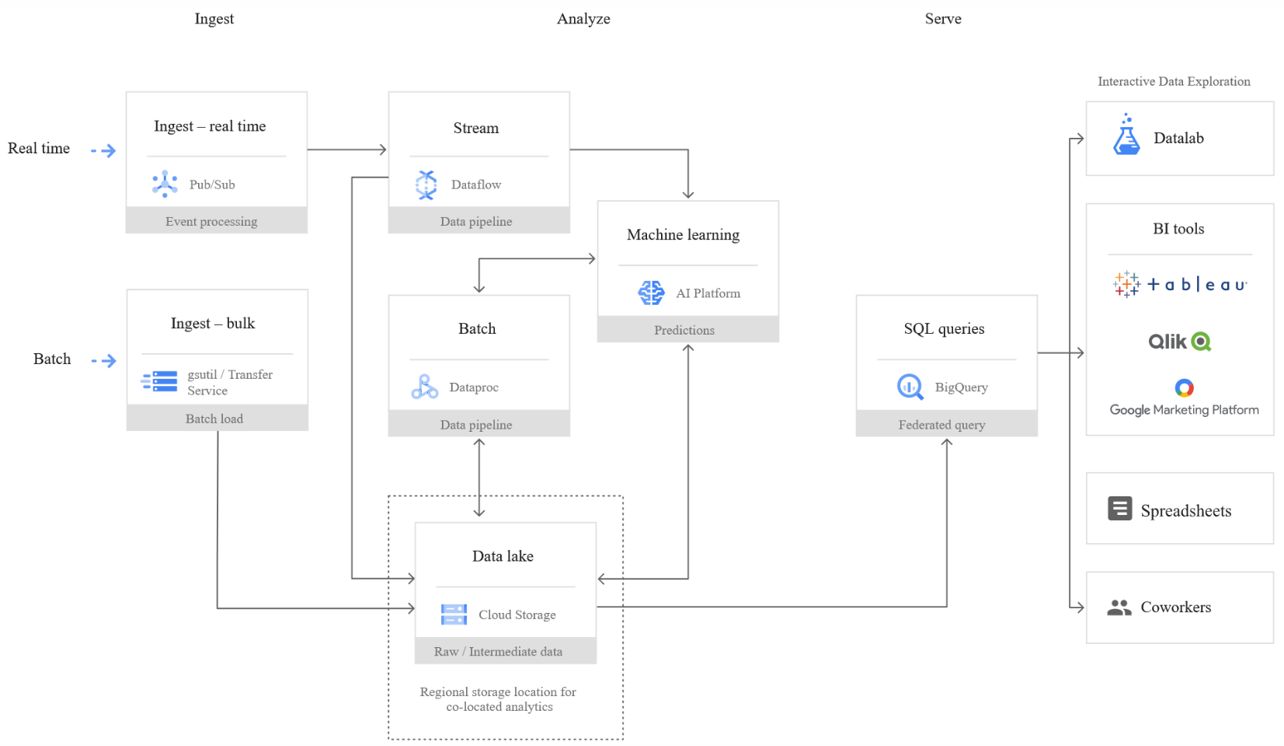
\includegraphics[height=.8\textheight]{imgs/gcpipeline.png}
\end{frame}



\ssec{Structural patterns for data pipelines}
\begin{frame}{Structural patterns}
Patterns are architectural solutions to problems in software design
\i Address common problems in software development
\si Command pattern
\si Messaging pattern
\si Priority queue pattern
% \si Fan-out pattern
\si Pipes and filters pattern
\end{frame}

\begin{frame}{Command pattern}
encapsulate a request as an object, thereby letting you parameterize clients with different requests, queue or log requests, and support undoable operations” because of the “need to issue requests to objects without knowing anything about the operation being requested or the receiver of the request”

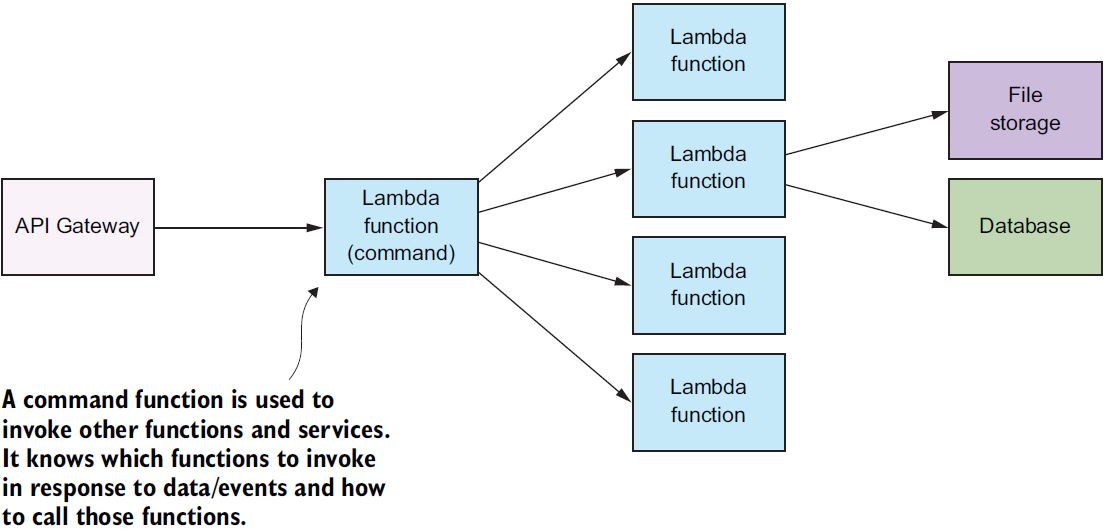
\includegraphics[scale=.4]{imgs/pattern_command.PNG}
\end{frame}

\begin{frame}[allowframebreaks]{Pipes and filters pattern}
Decompose a complex processing task into a sequence of manageable services
\i Components designed to transform data are referred to as filters
\i Connectors that pass data between components are referred to as pipes

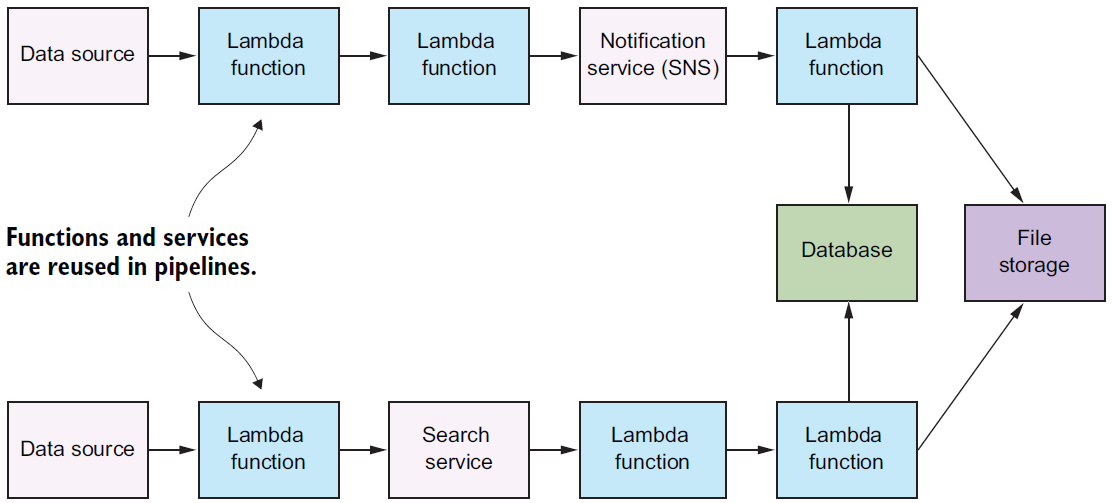
\includegraphics[width=.7\linewidth]{imgs/pattern_pipeline.PNG}
\end{frame}

\begin{frame}{Messaging pattern}
Decoupling functions and services from direct dependence on one another and allowing storage of events/records/requests in a queue. The reliability comes from the fact that if the consuming service goes offline, messages are retained in the queue and can still be processed at a later time.
\i Depending on how the system is designed, a message queue can have a single
sender/receiver or multiple senders/receivers.

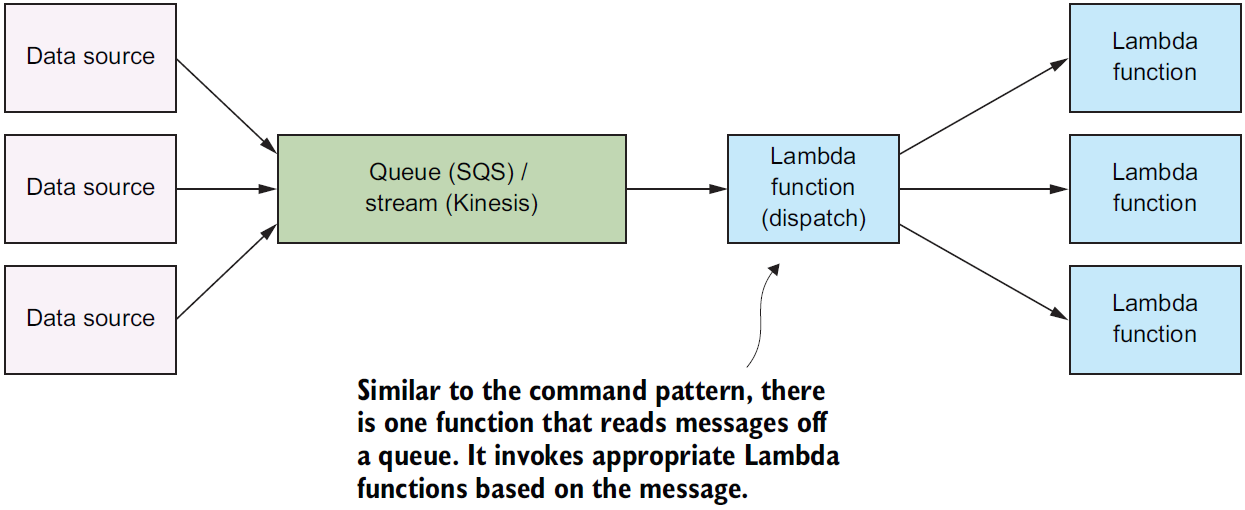
\includegraphics[scale=.4]{imgs/pattern_messaging.PNG}
\end{frame}

\begin{frame}{Priority queue pattern}
Control how and when messages are dealt with
\i Different queues, topics, or streams to feed messages to your functions 
\i High-priority messages go through expensive services with more capacity

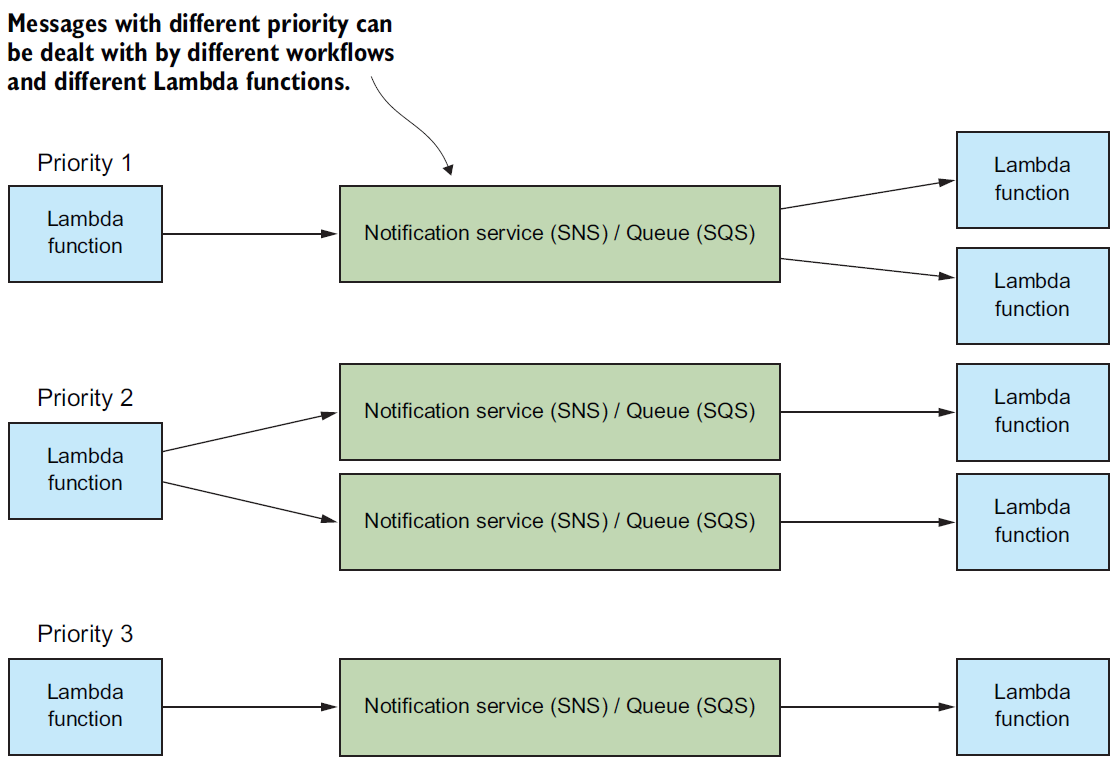
\includegraphics[scale=.4]{imgs/pattern_priority.PNG}
\end{frame}

\ssec{Event streams}
\begin{frame}{Key concepts}

\textbf{Event}: anything that we can observe occurring at a particular point in time

\textbf{Continuous streaming}: an illimitated succession of individual events, ordered by the point in time at which each event occurred

\textbf{Publish/subscribe (pub/sub)}: a way of communicating messages

\i Senders publish messages associated with one or more topics
\i Receivers subscribe to specific topics, receive all messages with that topic
\i Messages are events

\end{frame}

\begin{frame}{The unified log}

\begin{block}{Unified log}

Unified, append-only, ordered, distributed log that allows the centralization of continuous event streams

\end{block}

General idea:

\i Collect events from disparate source systems
\i Store them in a unified log
\i Enable data processing applications to operate on these event streams

\end{frame}

\begin{frame}{Features of a unified log}

\textbf{Unified}: a single deployment of this technology a company, with multiple applications sending events to it and reading events from it
  \i Log serves as central data backbone
  \i Unified log can contain many distinct continuous streams of events
  \si Not all events are sent to the same event stream

\textbf{Append-only}: new events are appended to the unified log
\i existing events are never updated in place
\i if read the event \#10, never look at events 1 through 10 again
\i Events are automatically deleted from the unified log when they age 
\end{frame}

\begin{frame}{Features of a unified log}
\textbf{Distributed}: the unified log lives across a cluster of machines

\i Still, the log is unified since we have a single (conceptual)
\i Scalability: work with streams larger than the capacity of single machines
\i Durability: replicate all events within the cluster to overcome data loss
\i Divide events in a given stream into *shards* (partitions)

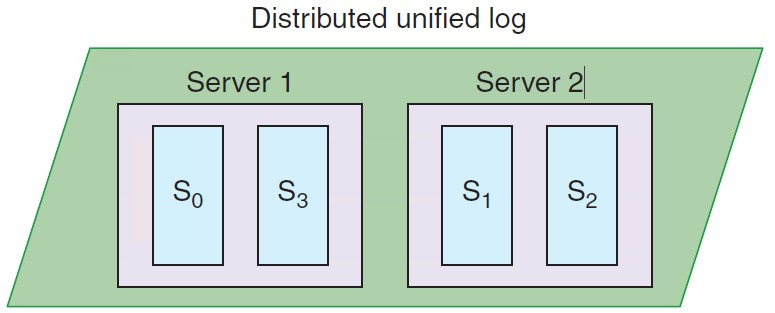
\includegraphics[width=.6\linewidth]{imgs/eventstream_shard.jpg}
\end{frame}

\begin{frame}{Features of a unified log}
\textbf{Ordered}: events in a shard have a sequential IDs (\textit{offset}, unique within a shard)
\i Local ordering keeps things much simpler
\i Applications maintain their own cursor for each shard
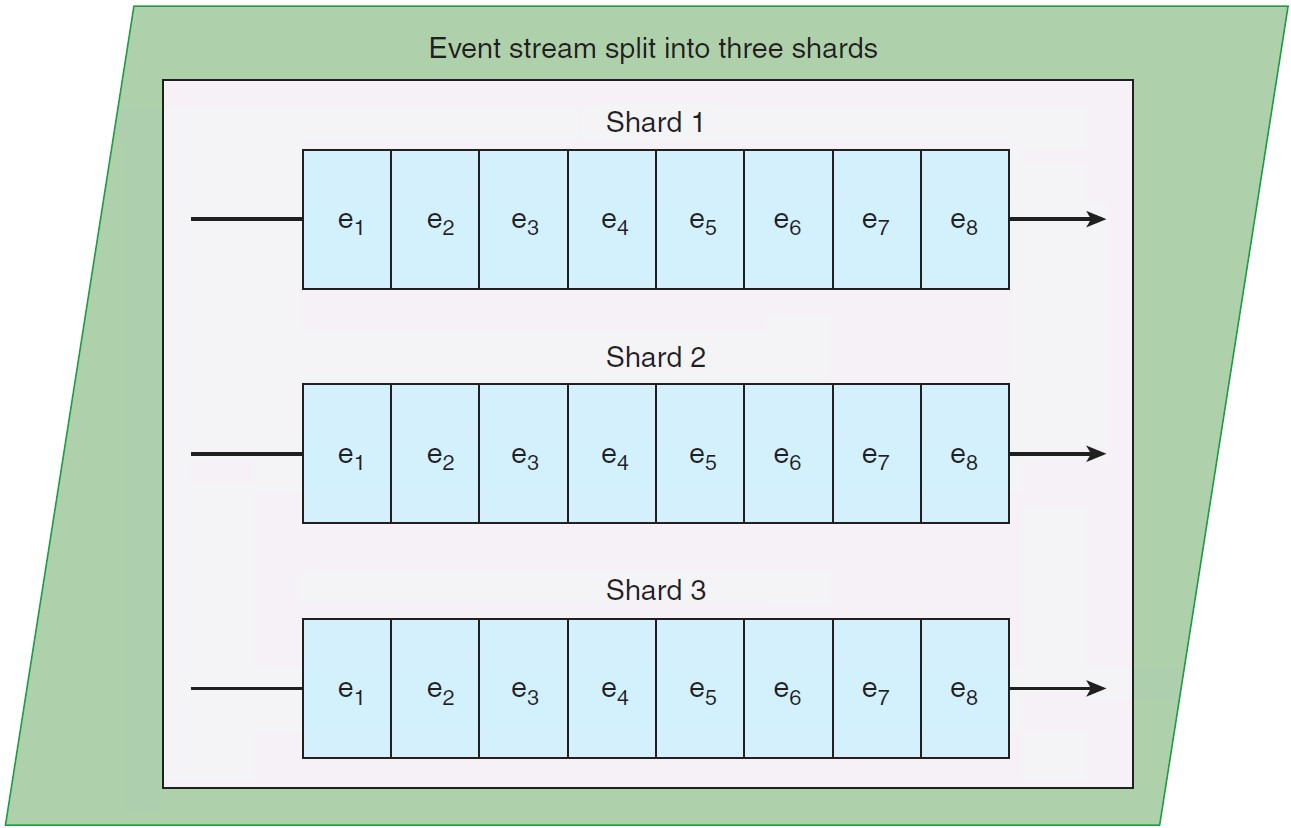
\includegraphics[width=.6\linewidth]{imgs/eventstream_order.jpg}
\end{frame}

\begin{frame}[allowframebreaks]{Event stream processing}
Two types of processing can be performed on a single event stream
\i \textbf{Single-event}, a single event produces zero or more events
\si \textit{Validating} "Does this event contain all the required fields?”
\si \textit{Enriching} "Where is this IP address located?"
\si \textit{Filtering} "Is this error critical?"
\i \textbf{Multiple-event}, multiple events collectively produce zero or more events
\si \textit{Aggregating}, functions such as minimum, maximum, sum
\si \textit{Pattern matching}, looking for patterns or co-occurence
\si \textit{Sorting}, reordering events based on a sort key
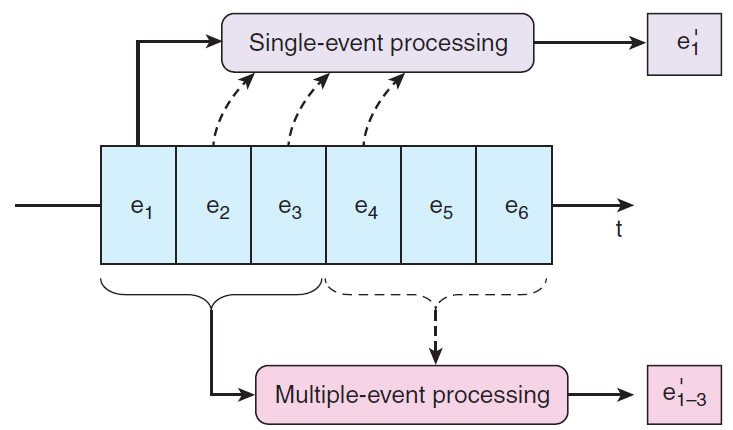
\includegraphics[width=.8\linewidth]{imgs/eventstream_processing.jpg}
\end{frame}


